% gebruik voor zowel figuren als tabellen de 'figure' environment. Op die manier delen ze de
% nummering, wat een CCN eis is. Tabel 3.1.2 volgt dan op figuur 3.1.1
\begin{figure}
    % figuren en tabellen hebben altijd een bovenschrift
    \caption{Gemiddelde afmeting per bloemonderdeel, plaatje gemaakt met highcharts}

    % direct na de caption zet je de label. Met \ref{fig:gemiddelde_afmeting} kan je vervolgens
    % naar deze figuur verwijzen in de tekst
    \label{fig:gemiddelde_afmeting_hc}

    % met \includegraphics kan je een figuur toevoegen
    % de linker kant van de figuur moet alignen met de caption. Gebruik \hspace{} om de figuur
    % zo te schuiven dat het goed is
    \hspace{-0.14cm}{
        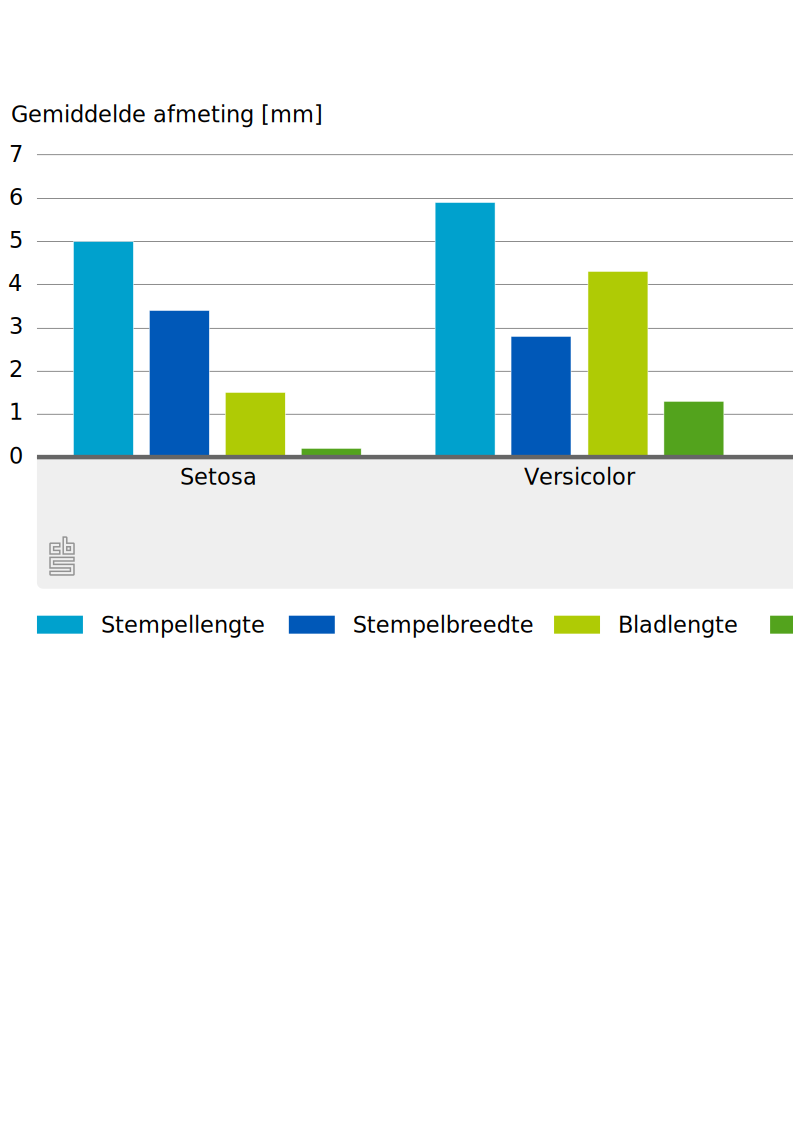
\includegraphics[width=\textwidth]{figures/iris_via_hc/afmetingen_bloem_hc}
    }
\end{figure}
